\begin{refsection}

\chapter{U--Th--(Sm)--He}\label{ch:UThHe}

\texttt{IsoplotR} offers a single input format for U--Th--(Sm)--He
data that can be captured by the following columns:

\begin{center}
He, err[He], U, err[U], Th, err[Th], Sm, err[Sm]
\end{center}

\noindent which contains all the necessary information to calculate
the age. Rewriting Equation~\ref{eq:U-Th-He}:
\begin{equation}
\begin{split}
  \left[^4\mbox{He}\right] = & ~a(t) 
   \mbox{[U]} + b(t)\mbox{[Th]} + c(t)\mbox{[Sm]} \\
   \mbox{where~} a(t) = &
   \left[8 \frac{137.818}{138.818} (e^{\lambda_{238}t} - 1) +
     7 \frac{1}{138.818} (e^{\lambda_{235}t} - 1) \right] \\
   b(t) = & ~6 (e^{\lambda_{232}t} - 1)\\
    \mbox{and~} c(t) = & ~0.1499 (e^{\lambda_{147}t} - 1)
\end{split}
\label{eq:UThHe2}
\end{equation}

Because Sm (1) produces only one \textalpha-particle per decay event;
(2) has a very long half-life; and (3) its radioactive isotope 147
only accounts for 14.99\% of total samarium, Sm can be ignored as a
parent in all but the most Sm-rich samples. For this reason, some
laboratories do not measure Sm at all, and the `Sm' and `err[Sm]'
columns are optional. If omitted, \texttt{IsoplotR} will simply assume
that the Sm-concentration is zero.\\

The He, U, Th (and Sm) measurements must be expressed in internally
consistent \textbf{atomic units} such as mol, fmol, pmol, mol/cc,
fmol/\textmu{g} etc. They must not be expressed in mass units such as
ppm, ppb or wt\%! For U and Sm, which are poly-isotopic elements, it
is the total amount that is required, and not just
\textsuperscript{238}U and \textsuperscript{147}Sm. A second important
requirement is that the data have been corrected for
\textbf{\textalpha-ejection} prior to analysis, as explained in the
next section.

\section{The \textalpha-ejection correction}\label{sec:alpha-ejection}

Helium, like argon, is a noble gas that is lost to the environment
(and eventually to space) at high temperatures by volume diffusion.
Additional complication is added by the physical separation of the
parent and daughter nuclides in the U-Th-(Sm)-He system. This
separation results from the energy released during \textalpha-decay,
which displaces the \textalpha-particles by up to 16~\textmu{m} and
may result in the ejection of helium produced by parent atoms that are
sited near the edges of the host mineral. That lost helium must be
taken into account when interpreting the thermal history of a
sample. For rapidly cooled samples, this can be done by applying a
geometric correction to the U, Th and Sm-measurements. For a sphere:
\begin{equation}
  F_T = 1 - \frac{3}{4}\frac{S}{R} + \frac{1}{16} \left[\frac{S}{R}\right]^3
    \label{eq:FTsphere}
\end{equation}

\noindent where $F_T$ is the fraction of helium that is retained in
the grain, $r$ is the radius of a sphere with equivalent
surface-to-volume ratio as the mineral habit of interest, and $S$ is
the \textalpha-stopping distance:

\begin{center}
\begin{tabular}{cccccc}
  mineral & \textsuperscript{238}U & \textsuperscript{235}U
  & \textsuperscript{232}Th & \textsuperscript{147}Sm \\ \hline
  apatite & 18.81 & 21.80 & 22.25 & 5.93 \\
  zircon & 15.55 & 18.05 & 18.43 & 4.76 \\
  sphene & 17.46 & 20.25 & 20.68 & 5.47
\end{tabular}
\captionof{table}{\textalpha-stopping distances ($S$) in \textmu{m}.}
\label{tab:stoppingdistances}
\end{center}

Most minerals are not spherical but elongated prismatic, and can be
approximated to a first degree as cylinders with radius $r$ and height
$h$:
\begin{equation}
  F_T = 1 - \frac{1}{2}\frac{(r+h)S}{rh} +
  0.2122 \frac{S^2}{rh} + 0.0153 \frac{S^3}{r^3}
  \label{eq:FTcylinder}
\end{equation}

An extensive list of formulas for even more realistic geometric shapes
is provided by \citet{ketcham2011}. The \textalpha-ejection correction
can be applied in one of three ways:

\begin{enumerate}
\item For relatively young ($<100$~Ma) samples, the ejected helium can
  be mathematically restored to a good approximation by dividing the
  uncorrected U--Th--He age by $F_T$ \citet{farley2002}:
  \begin{equation}
    t^* \approx \frac{t}{
      \frac{a(t)[U]}{a(t)[U]+b(t)[Th]}
      \left(
      \frac{137.818}{138.818} F_T^{238} +
      \frac{1}{138.818} F_T^{235}
      \right) + 
      \frac{b(t)[Th]}{a(t)[U]+b(t)[Th]} F_T^{232}
    }
    \label{eq:alphacorr1}
  \end{equation}

  \noindent where $t^*$ is the corrected age; $a(t)$ and $b(t)$ are
  defined in Equation~\ref{eq:UThHe2}; and $F_T^{238}$, $F_T^{235}$
  and $F_T^{232}$ are the \textalpha-retention factors of
  \textsuperscript{238}U, \textsuperscript{235}U and
  \textsuperscript{232}Th, respectively.
\item More accurate results are obtained by dividing not the age but
  the helium concentrations by the \textalpha-retention factor
  \citep{min2003, vermeesch2008a}:
  \begin{equation}
    [\mbox{He}^*] = \frac{[\mbox{He}]}{
      \frac{a(t)[\mbox{U}]}{a(t)[\mbox{U}]+b(t)[\mbox{Th}]}
      \left(
      \frac{137.818}{138.818} F_T^{238} +
      \frac{1}{138.818} F_T^{235}
      \right) + 
      \frac{b(t)[\mbox{Th}]}{a(t)[\mbox{U}]+b(t)[\mbox{Th}]} F_T^{232}
    }
    \label{eq:alphacorr2}
  \end{equation}
  \noindent and then plugging [He$^*$] into Equation~\ref{eq:UThHe2}
  instead of [He]. The difference between
  Equations~\ref{eq:alphacorr1} and \ref{eq:alphacorr2} can reach
  several percent for early Precambrian ages.
\item The most accurate approach to \textalpha-ejection correction is to
  adjust not the radiogenic daughter product but the radioactive
  parents:
  \begin{equation}
      [{}^{238}\mbox{U}^*] = \frac{[{}^{238}\mbox{U}]}{F_T^{238}},~
      [{}^{235}\mbox{U}^*] = \frac{[{}^{235}\mbox{U}]}{F_T^{235}},~
      \mbox{~and~} [{}^{232}\mbox{Th}^*] =
      \frac{[{}^{232}\mbox{Th}]}{F_T^{232}}
    \label{eq:alphacorr3}
  \end{equation}
  \noindent and then substituting [\textsuperscript{238}U$^*$],
            [\textsuperscript{235}U$^*$] and [\textsuperscript{232}Th$^*$]
            for [\textsuperscript{238}U], [\textsuperscript{235}U] and
            [\textsuperscript{232}Th] in Equation~\ref{eq:UThHe2}.
\end{enumerate}

\texttt{IsoplotR} assumes that the \textalpha-ejection correction has
been applied to the data \textbf{prior} to age calculation. This must
be done using either method 2 or 3 above.

\section{isochrons}

More often than not, and more often than for other geochronometers,
U-Th-(Sm)-He data are overdispersed with respect to the analytical
uncertainties. Several mechanisms have been invoked to explain this
overdispersion, including compositional effects, radiation damage, and
breakage during mineral separation.\\

\texttt{IsoplotR} implements four different ways to visualise, average
and quantify the overdispersion.  The first two of these are the
weighted mean and radial plot, which were discussed in
Sections~\ref{sec:weightedmean} and \ref{sec:radial}. The third way is
the isochron plot and age. This uses a first order approximation of
the U--Th--He age equation:
\begin{equation}
  t \approx \frac{\left[{}^{4}\mbox{He}\right]}{P} \mbox{,~where~} P =
  \left[8 \frac{137.818}{138.818} \lambda_{38} + 7 \frac{1}{138.818}
    \lambda_{35} \right] [\mbox{U}] + 6 \lambda_{32} [\mbox{Th}]
    \label{eq:t=HeP}
\end{equation}

\noindent which is accurate to better than 1\% for ages less than
100~Ma \citep{vermeesch2008a}. A U--Th--He isochron is constructed by
plotting the numerator of the right-hand side of
Equation~\ref{eq:t=HeP} against the denominator and fitting a straight
line through several aliquots of the same sample:\\

\noindent\begin{minipage}[t]{.4\linewidth}
\strut\vspace*{-\baselineskip}\newline
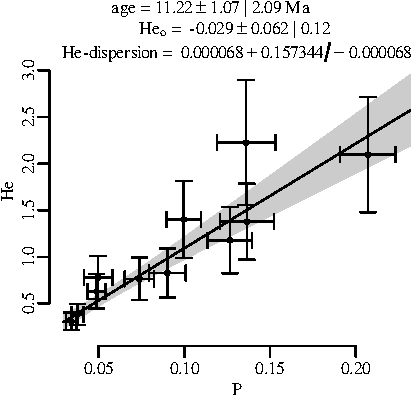
\includegraphics[width=\textwidth]{../figures/UThHeisochron.pdf}\\
\end{minipage}
\begin{minipage}[t]{.6\linewidth}
  \captionof{figure}{U--Th--He isochron with a model-3 fit. Because
    the parent and daughter nuclides are analysed separately on
    different mass spectrometers, their uncertainties are uncorrelated
    with each other. Hence the data are shown as error crosses instead
    of error ellipses.}
  \label{fig:UThHeisochron}
\end{minipage}

\section{Compositional data analysis and the `helioplot'}
\label{sec:UThHeCompositional}

The fourth and final way to visualise and average U--Th--He data is
based on the fact that U, Th and He are \emph{compositional}
data. This means that it is not so much the absolute concentrations of
these elements that bear the chronological information, but rather
their relative proportions. Equation~\ref{eq:UThHe2} can be recast in
terms of the elemental ratios U/He, Th/He, which take on strictly
positive values:
\begin{equation}
  a(t) \frac{[\mbox{U}]}{[\mbox{He}]} +
  b(t) \frac{[\mbox{Th}]}{[\mbox{He}]} = 1
\end{equation}

The space of all possible U--Th--He compositions fits within the
constraints of a ternary diagram. If Sm is included as well, then this
expands to a three-dimensional tetrahedral space
\citep{vermeesch2008a}. The \textbf{central age} is obtained by first
computing the average U--Th--He composition of a multi-sample dataset,
and then calculating the U--Th--He corresponding to that composition.
This is a similar procedure to the two-step process that was used to
compute concordia ages in Section~\ref{sec:concordia}.  Unfortunately,
averaging compositional data is not as straightforward as one may
think. Consider, for example, the following ternary dataset:\\

\noindent\begin{minipage}[t]{.4\linewidth}
\strut\vspace*{-\baselineskip}\newline
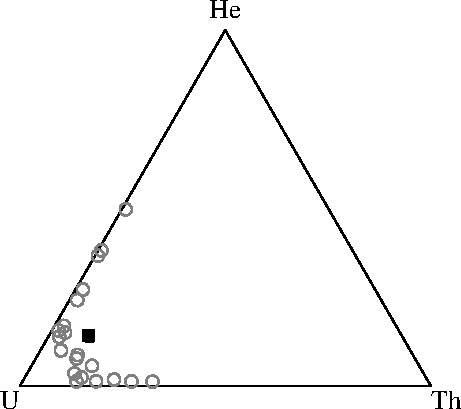
\includegraphics[width=\textwidth]{../figures/ternaryhelium.pdf}\\
\end{minipage}
\begin{minipage}[t]{.6\linewidth}
  \captionof{figure}{The U--Th--He age equation is scale invariant in
    the sense that the three elements can be renormalised to unity
    without loss of chronological information. This figure shows a
    synthetic dataset of 20 scattered U--Th--He measurements (grey
    circles). The arithmetic mean composition of the dataset is shown
    as a black square. It plots outside the data cloud, and is
    therefore not representative of the data.\\}
  \label{fig:ternaryhelium}
\end{minipage}

\citet{aitchison1986} showed that the natural way to process
compositional data is by subjecting them to a \textbf{logratio
  transformation}. In the case of the U--Th--He system, the logratio
analysis is achieved by first defining two new variables:
\begin{equation}
  u \equiv \ln\!\left(\frac{\mbox{[U]}}{\mbox{[He]}}\right),
  v \equiv \ln\!\left(\frac{\mbox{[Th]}}{\mbox{[He]}}\right)
  \label{eq:alr}
\end{equation}

\noindent and then performing the desired statistical analysis
(averaging, uncertainty propagation, ...) on the transformed
data. Upon completion of the mathematical operations, the results can
then be mapped back to U-Th-(Sm)-He space using an inverse logratio
transformation:
\begin{equation}
    [He] = \frac{1}{\left[e^{u}+e^{v}+1\right]},~
    [U] = \frac{e^{u}}{\left[e^{u}+e^{v}+1\right]},~
    [Th] = \frac{e^{v}}{\left[e^{u}+e^{v}+1\right]}
    \label{eq:ialr}
\end{equation}

\noindent where [He] + [U] + [Th] = 1.\\

\noindent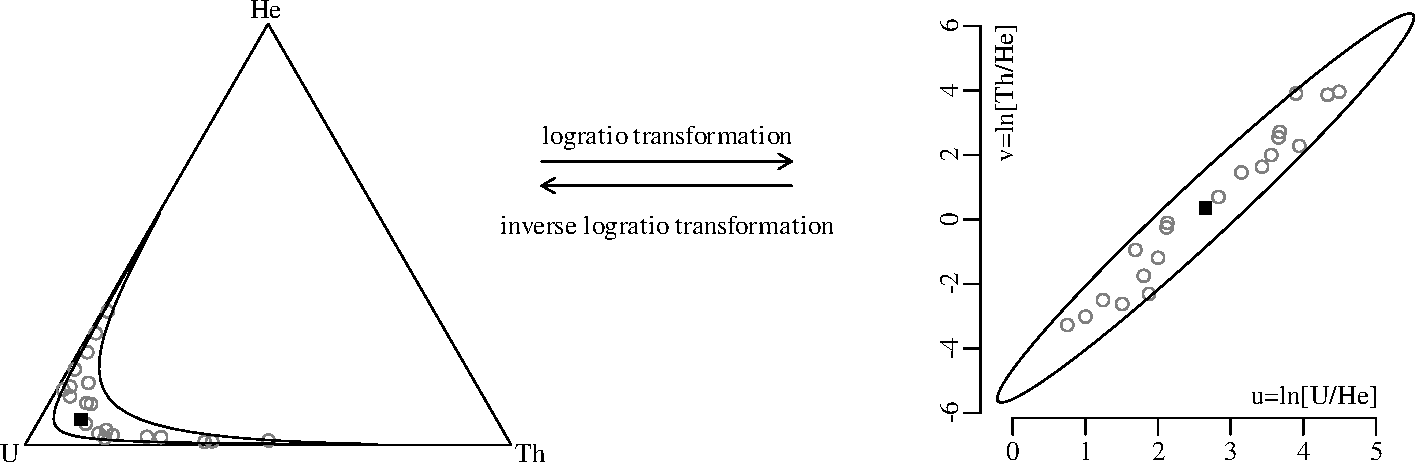
\includegraphics[width=\linewidth]{../figures/alr.pdf}
\begingroup
\captionof{figure}{The logratio transformation maps data from an
  $n$-dimensional compositional space to an $(n-1)$-dimensional
  Euclidean space. For the U--Th--He data, it maps the data from a
  ternary diagram ($n=3$) to a bivariate ($n-1=2$) dataspace using
  Equation~\ref{eq:alr}. In this transformed space, it is safe to
  calculate the arithmetic mean (black square) and confidence regions
  (black ellipse). After completion of these calculations, the result
  can be mapped back to the ternary diagram using the inverse logratio
  transformation (Equation~\ref{eq:ialr}).\\}
\label{fig:alr}
\endgroup

In the context of U--Th--He dating, the central age is defined as the
age that corresponds to the arithmetic mean composition in logratio
space. \texttt{IsoplotR}'s \texttt{helioplot} function performs this
calculation using the same algorithm that is used to obtain the
weighted mean U-Pb composition for the concordia age calculation
(Section~\ref{sec:concordia}).\\

\noindent\begin{minipage}[t]{.7\linewidth}
\strut\vspace*{-\baselineskip}\newline
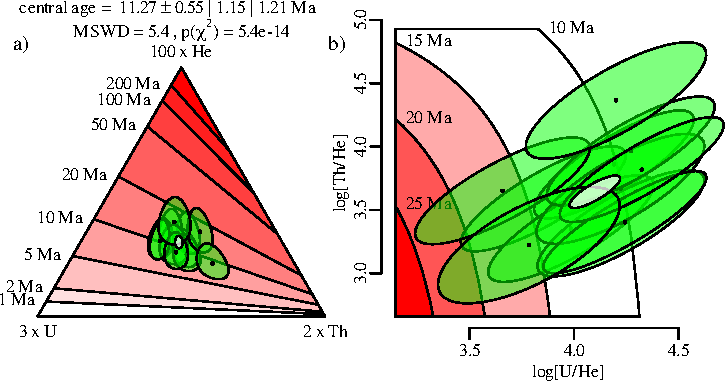
\includegraphics[width=\textwidth]{../figures/helioplot.pdf}\\
\end{minipage}
\begin{minipage}[t]{.3\linewidth}
  \captionof{figure}{a) ternary diagram and b) logratio diagram or
    `helioplot' of the U--Th--He data from
    Figure~\ref{fig:UThHeisochron}. The white ellipse marks the
    average U--Th--He composition.\\}
  \label{fig:UThHeIsochronHelioplot}
\end{minipage}

Overdispersion is treated similarly as in a regression context
(Section~\ref{sec:regression}).  Thus, there are options to augment
the uncertainties with a factor $\sqrt{\mbox{MSWD}}$ (model-1); to
ignore the analytical uncertainties altogether (model-2); or to add an
overdispersion term to the analytical uncertainties (model-3).  The
helioplot diagram provides a convenient way to simultaneously display
the isotopic composition of samples and their chronological
meaning. In this respect, they fulfil the same purpose as the U--Pb
concordia diagram (Section~\ref{sec:concordia}) and the U--series
evolution plot (Section~\ref{sec:ThUevolution}).

\printbibliography[heading=subbibliography]

\end{refsection}
